% THIS IS SIGPROC-SP.TEX - VERSION 3.1
% WORKS WITH V3.2SP OF ACM_PROC_ARTICLE-SP.CLS
% APRIL 2009
%
% It is an example file showing how to use the 'acm_proc_article-sp.cls' V3.2SP
% LaTeX2e document class file for Conference Proceedings submissions.
% ----------------------------------------------------------------------------------------------------------------
% This .tex file (and associated .cls V3.2SP) *DOES NOT* produce:
%       1) The Permission Statement
%       2) The Conference (location) Info information
%       3) The Copyright Line with ACM data
%       4) Page numbering
% ---------------------------------------------------------------------------------------------------------------
% It is an example which *does* use the .bib file (from which the .bbl file
% is produced).
% REMEMBER HOWEVER: After having produced the .bbl file,
% and prior to final submission,
% you need to 'insert'  your .bbl file into your source .tex file so as to provide
% ONE 'self-contained' source file.
%
% Questions regarding SIGS should be sent to
% Adrienne Griscti ---> griscti@acm.org
%
% Questions/suggestions regarding the guidelines, .tex and .cls files, etc. to
% Gerald Murray ---> murray@hq.acm.org
%
% For tracking purposes - this is V3.1SP - APRIL 2009

%\documentclass{acm_proc_article-sp}
\documentclass{sig-alternate-10pt}
\usepackage{graphicx}

\begin{document}

%\title{A Sample {\ttlit ACM} SIG Proceedings Paper in LaTeX
\title{Large-scale Linear Optimization through Machine Learning}
%Format\titlenote{(Does NOT produce the permission block, copyright information nor page numbering). For use with ACM\_PROC\_ARTICLE-SP.CLS. Supported by ACM.}}

%\subtitle{[Extended Abstract]
%\titlenote{A full version of this paper is available as
%\textit{Author's Guide to Preparing ACM SIG Proceedings Using
%\LaTeX$2_\epsilon$\ and BibTeX} at
%\texttt{www.acm.org/eaddress.htm}}}

%
% You need the command \numberofauthors to handle the 'placement
% and alignment' of the authors beneath the title.
%
% For aesthetic reasons, we recommend 'three authors at a time'
% i.e. three 'name/affiliation blocks' be placed beneath the title.
%
% NOTE: You are NOT restricted in how many 'rows' of
% "name/affiliations" may appear. We just ask that you restrict
% the number of 'columns' to three.
%
% Because of the available 'opening page real-estate'
% we ask you to refrain from putting more than six authors
% (two rows with three columns) beneath the article title.
% More than six makes the first-page appear very cluttered indeed.
%
% Use the \alignauthor commands to handle the names
% and affiliations for an 'aesthetic maximum' of six authors.
% Add names, affiliations, addresses for
% the seventh etc. author(s) as the argument for the
% \additionalauthors command.
% These 'additional authors' will be output/set for you
% without further effort on your part as the last section in
% the body of your article BEFORE References or any Appendices.

\numberofauthors{1} %  in this sample file, there are a *total*
% of EIGHT authors. SIX appear on the 'first-page' (for formatting
% reasons) and the remaining two appear in the \additionalauthors section.
%
\author{
% You can go ahead and credit any number of authors here,
% e.g. one 'row of three' or two rows (consisting of one row of three
% and a second row of one, two or three).
%
% The command \alignauthor (no curly braces needed) should
% precede each author name, affiliation/snail-mail address and
% e-mail address. Additionally, tag each line of
% affiliation/address with \affaddr, and tag the
% e-mail address with \email.
%
% 1st. author
\alignauthor
JungAh Hong\\%\titlenote{Dr.~Trovato insisted his name be first.}\\
       \affaddr{20143729}\\
%       \email{trovato@corporation.com}
}

\maketitle
%
\begin{abstract}
aaa
\end{abstract}

% A category with the (minimum) three required fields
%\category{H.4}{Information Systems Applications}{Miscellaneous}
%A category including the fourth, optional field follows...
%\category{D.2.8}{Software Engineering}{Metrics}[complexity measures, performance measures]

%\terms{Theory}

%\keywords{ACM proceedings, \LaTeX, text tagging} % NOT required for Proceedings

\section{Introduction}

Recent advances in cloud and distributed computing enabled Big Data 
processing. Today, processing big data generally falls under the category 
of statistical inferencing, e.g., predicting congestion with traffic data 
in the road network. The bottleneck is mainly the system I/O capacity for 
reading and writing data. The computation applied to individual items is 
relatively simple compared to the amount of data to process. 

However, big data processing will ultimately require large scale 
optimizations in the future. For example, one might want to optimize the 
traffic light system of an entire city using predictions. 
Unfortunately, the traditional optimization algorithms are fundamentally hard to parallelize. These algorithms are hard to scale and cannot run on existing cloud environment. 

In recent years, several abstractions using belief propagation (BP), a popular class of distributed machine learning algorithm, to 
parallelize linear optimizations have been proposed~\cite{BPLP, BPLPmatching}. 
Several well known optimization problems - the matching problem~\cite{BPmatching} and min-cost network flow problem~\cite{BPflow} - were relaxed to a Linear Program (LP) then solved through BP in certain cases. 

The goal of this research is to develop a practical system that runs on modern cloud environments, such as Amazon EC2, for parallel, distributed optimizations on maximum weight matching (MWM) problems. 
We plan to enhance recent theoretical developments on BP for large-scale linear optimizations and and develop a cloud-based software to solve MWM problems using the power of large-scale cloud computing.


\section{Background}

\subsection{Belief Propagation}
Belief Propagation is a message passing algorithm
for performing inference on graphical models. It is common used in artificial intelligence and information theory and has demonstrated empirical success in numerous applications.

On the graph, messages are associated on each edge with each direction and updated until convergence.
Each node has a \textbf{belief}, which is calculated from incoming messages. 
Those beliefs are used as decision variable of nodes and edges. 

%\subsection{Weighted matching and its LP relaxation}
%\subsection{Max-product for weighted matching}
\subsection{Simplified Max-product for weighted matching~\cite{BPLPmatching}}
Let $m_{i \rightarrow j}$ denote the messsage at time $t$, node $i$ and edge $e in E_i$. 
For every pair of neighbors $i$ and $j$, let $e = (i, j)$ be the edge connecting the two,
and define 
\begin{displaymath}
a_{i \rightarrow j}^t = log(\frac{m_{i \rightarrow e}^t[0]}{m_{i \rightarrow e}^t[1]})
\end{displaymath}

\begin{itemize}
\item

%\begin{displaymath}\int^b_af(t)dt = G(b) - G(a).\end{displaymath}
%\begin{equation}\sum_{i=0}^{\infty}x_i=\int_{0}^{\pi+2} f\end{equation}

\textbf{(INIT)} Set $t$=0 and initialize each $a_{i \rightarrow j}^0$ = 0
\item
\textbf{(ITER)} Iteratively compute new messages until convergence as follows: ($y_+$ = max(0, $y$))
\begin{displaymath}
a_{i \rightarrow j}^{t+1} = max_{k \in N(i)-j} (w_{ik} - a_{k \rightarrow i}^{t})_+
\end{displaymath}
\item
\textbf{(ESTIM)} Upon convergence, output estimate $\hat{x}_{(i,j)}$ is, respectively, >, <, or = $w_{ij}$.
\end{itemize}

It guarantees convergence when the extreme points of the matching LP polytope are integral. In other words, if LP doesn't have any fractional optima. 


\subsection{Hungarian algorithm~\cite{wiki_hungarian}}
The Hungarian algorithm is a combinatorial optimization algorithm that solves the assignment problem in polynomial time. 
The time complexity of the original algorithm was $O(n^4)$, modified to achieve $O(n^3)$ running time. 

If we formulate the problem using a bipartite graph, $G=(S, T;E)$ with $n$ vertices on one side ($S$) and same number of vertices on the other side ($T$), and each edge has a nonnegative weight $w(i, j)$, the way to find a perfect matching with minimum cost is as below. (Edges with 0 weight are added to make the graph complete in advance)

Let $y:(S \cup T) \mapsto \Re$ a \textbf{potential} if $y(i) + y(j) \leq c(i,j)$ for each $i \in S, j \in T$.
The value of potential $y$ is $\sum_{v \in S \cup T}^{y(v)}$. The Hungarian method finds a perfect matching of tight edges: an edge $ij$ is called tight for a potential $y$ if $y(i) + y(j) = c(i,j)$. Let $G_y$ denote the subgraph of tight edges. The cost of a perfect matching in $G_y$ equals the value of $y$.

\subsection{Blossom algorithm~\cite{wiki_blossom}}
The blossom algorithm is an algorithm for constructing maximum matchings on graphs.
The matching is constructed by iteratively improving an initial empty matching along augmenting paths in the graph. 
Micali and Vazirani~\cite{blossom} showed an algorithm that constructs maximum matching in $O(|E||V|^{1/2})$ time.



\section{Design}

\begin{figure*}
\centering
%\includegraphcs[width=1.0\columnwidth]{system.pdf}
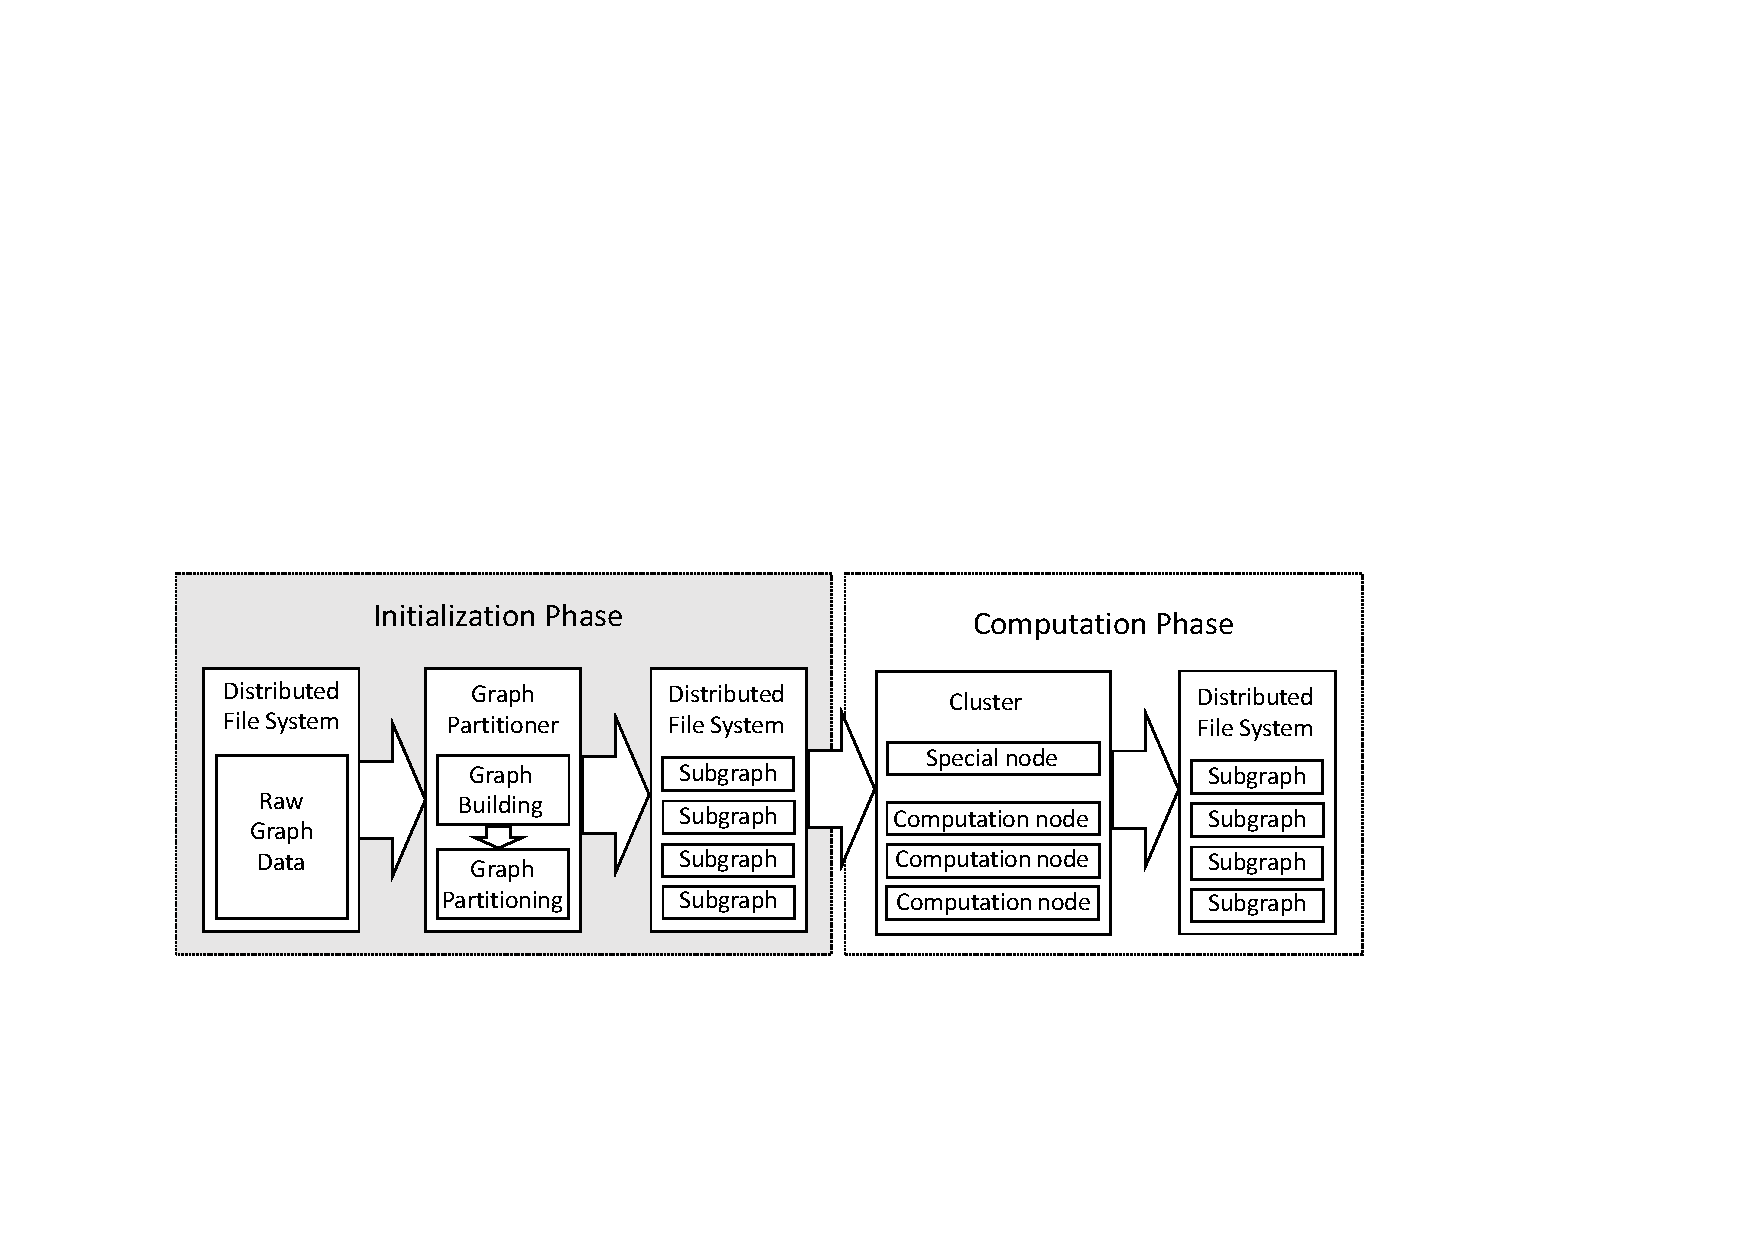
\psfig{file=system.pdf, height=2in, width=6.5in}
\caption{A high level overview of the system}
%\tightcaption{aaaa}
\label{fig:cdn}
\end{figure*}

\subsection{Distributed data graph}
Efficiently partitioning the data graph in the distributed environment requires balancing computation, communication, and storage. 
Therefore, we need to construct balanced subgraphs that minimize number of edges/nodes that cross between machines. 

PowerGraph achieves balanced partitioning by considering the strongest feature of natural graphs: having highly skewed power-law degree distributions.~\cite{powerGraph} 
We used the same partitioning strategy and stored each part as a separate file on a distributed storage system (e.g., HDFS, Amazon S3).

\subsection{Configuration management}
The system needs management during the computation. 
At initialization phase, the graph is torn down to several atom graphs and mapped to each machines. 
Machines are assigned by ZooKeeper. A subset of nodes are assigned to particular tasks (e.g., shared data table), while the remaing nodes are assigned to do the computation. 
Some idle nodes remains in a pool which can be used as needed (e.g., a node might registered as a stanby for multiple active nodes). 

ZooKeeper maintains overall system status and stays reliable when the fault occurs. Thus, the system would remain safe over the fault management by ZooKeeper.

%\subsection{
\subsection{Scheduler}
The scheduler represents a dynamic list of tasks to be executed. Since new messages are calculated from the previous incoming messages, if a message is updated, the messages on the connected edges need update as well. 

The schedule management is also designed with ZooKeeper. ZooKeeper maintains consistency between parallel updates with distributed locks. 
The computation iterates until convergence. ZooKeeper terminates the computation from all the nodes when the system reaches convergence. 


\subsection{System design}
In Fig. 1, we provide a high-level overview of the system. 
The computation begins by constructing subgraph representation on a Distributed File System (DFS). 
%Fig. provides the high-level overview of the computation engine. 

Each instance is executed on each machine. 
Some nodes are assigned to particular tasks and the rest of them are assigned to computation. 


\section{Conclusions}

%We identified several limitations in existing optimization algorithms. 
We idntified the limitation in existing optimization algorithms that they're structurally not parallelizable. We used BP, a message passing machine learnng algorithm has parallel structure, to solve the MWM problem in distributed environment. 

The abstraction uses a \textbf{data graph} as a computational model. Updates are done with the local computation on each vertex. Parallel \textbf{scheduler} manages the scheduling of dynamic iterative parallel computation.  

To manage the task/graph assignment, scheduler and faults we used ZooKeeper, the service enables easier management of distributed configuration and synchronization. 

Since ZooKeeper makes dns-based assignment, the load balancing still remains challenging. 


%\end{document}  % This is where a 'short' article might terminate



%
% The following two commands are all you need in the
% initial runs of your .tex file to
% produce the bibliography for the citations in your paper.
\bibliographystyle{abbrv}
\bibliography{sigproc}  % sigproc.bib is the name of the Bibliography in this case
% You must have a proper ".bib" file
%  and remember to run:
% latex bibtex latex latex
% to resolve all references
%
% ACM needs 'a single self-contained file'!
%
%\balancecolumns
%\balancecolumns
\end{document}
